% Search for all the places that say "PUT SOMETHING HERE".


\documentclass[11pt]{article}
\usepackage{amsmath,textcomp,amssymb,geometry,graphicx,tkz-graph}

\def\Name{Ben Augarten}  % Your name
\def\Sec{106}  % Your discussion section
\def\Login{cs170-bo} % Your login

\def\pm{\begin{pmatrix}}
\def\epm{\end{pmatrix}}

\title{CS170--Fall 2012 --- Solutions to Homework 3}
\author{\Name, section \Sec, \texttt{\Login}}
\markboth{CS170--Spring 2012 Homework 3 \Name, section \Sec}{CS170--Spring 2012 Homework 3 \Name, section \Sec, \texttt{\Login}}
\pagestyle{myheadings}

\begin{document}
\maketitle

\begin{enumerate}
\item
\begin{enumerate}
\item Once we receive the impulse response, we respond with a constant value, $\frac{1}{t_0}$ for a constant amount of time, $t_0$, and then output 0 from then on.
\item $c_k = \sum_{i=0}^k a_i b_{k-i}$, so between $0$ and $t_0$, $c_i=a_0*b_i=b_i$ because $a_j = 0$, $j \neq 0$ and $a_0=1$. We know $c_i=\frac{1}{t_0}$, for $0 \le i \le t_0$ and $0$ elsewhere, so for each coefficient of $b$, $b_i=\frac{1}{t_0}$, $0 \le i \le t_0$, else $b_i=0$. $b(x)=t_0+t_0x+...+t_0x^{t_0}$
\end{enumerate}
\newpage
\item
\begin{enumerate}
\item I'm going to use the formula for FFT in the textbook, which ignores the polynomial application of the algorithm and instead focuses on the transformation of basis.

We have two tuples, $(1,1,0,0)$, $(1,0,1,0)$, $\omega=e^{\pi i/2}$
\begin{align*}
(s_0,s_1)=\text{FFT}((1,0), e^{\pi i})&(s_0',s_1')=\text{FFT}((1,0), e^{\pi i})\\
(r_0,r_1,r_2,r_3)&=(s_0+s_0',s_1+i*s_1',s_0-s_0',s_1-i*s_1')\\
(s_0,s_1)&=\text{FFT}((1,0), e^{\pi i})\\
s_{00} = \text{FFT}((1), 1)&s_{00}' = \text{FFT}((0), 1)\\
S_{00} = 1&s_{00}'=0\\
(s_0,s_1)=(r_{00},r_{01})&=(1,1)\\
(s_0',s_1')=\text{FFT}((1,0), e^{\pi i})&=(1,1)\\
(r_0,r_1,r_2,r_3)&=(2,1+i,0,1-i)
\end{align*}
\begin{align*}
(s_0,s_1)=\text{FFT}((1,1), e^{\pi i})&(s_0',s_1')=\text{FFT}((0,0), e^{\pi i})\\
(r_0,r_1,r_2,r_3)&=(s_0+s_0',s_1+i*s_1',s_0-s_0',s_1-i*s_1')\\
(s_0,s_1)&=\text{FFT}((1,1), e^{\pi i})\\
s_{00} = \text{FFT}((1), 1)&s_{00}'=\text{FFT}((1), 1)\\
(s_{00}, s_{00}')&=(1,1)\\
(s_0,s_1)=(r_{00},r_{01})&=(2,0)\\
(s_0',s_1')=\text{FFT}((0,0), e^{\pi i})&=(0,0)\\
(r_0,r_1,r_2,r_3)&=(2,0,2,0)
\end{align*}
$(2,1+i,0,1-i)*(2,0,2,0)=(4,0,0,0)$
\begin{align*}
\text{FFT}((4,0,0,0), e^{- \pi i/2})\\
(s_0,s_1)=\text{FFT}((4,0), e^{-pi / 2})&(s_0',s_1')=\text{FFT}((0,0), e^{-\pi i/2})\\
(r_0,r_1,r_2,r_3)&=(s_0+s_0',s_1-i*s_1',s_0-s_0',s_1+i*s_1')\\
(s_0, s_1)&=\text{FFT}((4,0), -1)\\
s_{00}=\text{FFT}((4), 1)&s_{00}'=\text{FFT}((0),1)\\
(s_{00},s_{00}')=(4,0)\\
(s_0,s_1)=(r_{00},r_{01})=(4,4)\\
(s_0',s_1')=\text{FFT}((0,0), -1)&=(0,0)\\
(r_0,r_1,r_2,r_3)&=(4,4,4,4)\\
\end{align*}
$\frac{1}{4}(4,4,4,4)=(1,1,1,1)=1+x+x^2+x^3$\\
Now calculate using $(1,1,2,0)$ and $(2,3,0,0)$
\begin{align*}
(s_0,s_1)=\text{FFT}((1,2), e^{\pi i})&(s_0',s_1')=\text{FFT}((1,0), e^{\pi i})\\
(r_0,r_1,r_2,r_3)&=(s_0+s_0',s_1+i*s_1',s_0-s_0',s_1-i*s_1')\\
(s_0,s_1)&=\text{FFT}((1,2), 1)\\
s_{00}=\text{FFT}((1),1)&s_{00}'=\text{FFT}((2),1)\\
(s_{00},s_{00}')&=(1,2)\\
(s_0,s_1)=(r_{00},r_{01})&=(3,-1)\\
(s_0',s_1')&=(1,1)\text{ by part (a)}\\ 
(r_0,r_1,r_2,r_3)&=(4,-1+i,2,-1-i)\\
\end{align*}
\begin{align*}
(s_0,s_1)=\text{FFT}((2,0), e^{\pi i})&(s_0',s_1')=\text{FFT}((3,0), e^{\pi i})\\
(r_0,r_1,r_2,r_3)&=(s_0+s_0',s_1+i*s_1',s_0-s_0',s_1-i*s_1')\\
(s_0,s_1)&=\text{FFT}((2,0), 1)\\
s_{00}=\text{FFT}((2),1)&s_{00}'=\text{FFT}((0),1)\\
(s_{00},s_{00}')&=(2,0)\\
(s_0,s_1)=(r_{00},r_{01})&=(2,2)\\
(s_0',s_1')&=(3,3)\text{ same process as above}\\ 
(r_0,r_1,r_2,r_3)&=(5,2+3i,-1,2-3i)\\
\end{align*}
$(4,-1+i,2,-1-i)*(5,2+3i,-1,2-3i)=(20,-5-i,-2,-5+i)$\\
\begin{align*}
\text{FFT}((20,-5-i,-2,-5+i), e^{- \pi i/2})\\
(s_0,s_1)=\text{FFT}((20,-2), e^{-pi / 2})&(s_0',s_1')=\text{FFT}((-5-i,-5+i), e^{-\pi i/2})\\
(r_0,r_1,r_2,r_3)&=(s_0+s_0',s_1-i*s_1',s_0-s_0',s_1+i*s_1')\\
(s_0, s_1)&=\text{FFT}((20,-2), -1)\\
s_{00}=\text{FFT}((20), 1)&s_{00}'=\text{FFT}((-2),1)\\
(s_{00},s_{00}')&=(20,-2)\\
(s_0,s_1)=(r_{00},r_{01})&=(18,22)\\
(s_0', s_1')&=\text{FFT}((-5-i,-5+i), -1)\\
s_{10}=\text{FFT}((-5-i), 1)&s_{10}'=\text{FFT}((-5+i),1)\\
(s_{10},s_{10}')&=(-5-i,-5+i)\\
(s_0',s_1')=(r_{10},r_{11})&=(-10,-2i)\\
(r_0,r_1,r_2,r_3)&=(8,20,30,24)\\
\end{align*}
$\frac{1}{4}*(8,20,28,24)=(2,5,7,6)=2+5x+7x^2+6x^3$
\end{enumerate}
\newpage
\item
We need to find a path through $G$ that touches every vertex exactly once. We can use a topological sort such that any directed edge between any two vertices only points to a higher numbered vertex. Let the path start at the lowest numbered vertex, $v$. If it didn't start at $v$, then the path would never get to $v$ (no vertex can point to it). Now we follow the edge to the next highest order -- if it didn't then again there wouldn't be a way to get back to this vertex, and continue. For example, for each vertex with order from $1$ to $|G|$, called $v_1$ with ordering $i$ , get the vertex with ordering $i+1$, vertex $v_2$ , if $v_1\to v_2$ exists, then continue to $i+1$, if it doesn't exist then there is no path that touches every vertex exactly once.\\
Runtime: the topological sorting takes $\Theta(|V|+|E|)$, and looping over all of the vertices and edges takes again $O(|V|+|E|)$, so the entire algorithm is $O(|V|+|E|)$
\newpage
\item
\begin{enumerate}
\item We start by showing that if a graph $G$ has a eulerian tour then every vertex must have even degree. This is very easy to see. We start at any given vertex $v$, and follow an edge $(v,u)$ to $u$. In order to eventually get back to $v$ (we cannot use the same edge twice), there must be a matching inward edge that we can travel on. For every edge that leaves $v$ there must be an edge coming back in so we can eventually end at $v$. Lets call the matching edge back in edge $(w,v)$. Likewise, from $w$ we need an inward edge in order to get there in the tour, making $w$'s degree even because $w$ too needs an inward edge for every outward edge (or vice versa). We can continue matching these edges (note that $w$ could equal $v$ or $u$, and even in that case all would have even degrees) until we finally realize the full tour and have matched inward and outward edges at each vertex, verifying that each vertex has even degree.\\
Now we have to prove the converse -- if all vertices have even degree then the graph has an Eulerian tour. Lets pick a vertex to start at, and keep following edges until we arrive back at the starting vertex. We will arrive at the starting vertex because any walk that starts and ends on different vertices needs to have two vertices of odd degree (the start and end vertices) because the start vertex needs one more edge to follow out and the end vertex needs one more edge to follow in. Because there are no odd degree vertices in the graph, we must start and end our arbitrary walk on the same vertex. However, we could have missed an arbitrary amount of closed walks. All of the closed walks we missed are Eulerian tours of the subgraph because we can repeat the previous procedure, walking on that graph and ending at the same point that we started, and so we can just add them to the existing tour without problem. Thus the addition of the tours produces a complete Eulerian tour around the graph $G$.
\item An undirected graph has an Eulerian path that doesn't start and end on the same vertex iff all of its vertices have even degree except two with odd degree. Start with an Eulerian that starts and ends on different nodes, we pick the starting vertex of the Eulerian path, vertex $v$. Go from $v$ and traverse along the path. Every node in the middle of the path must be of even degree because the path enters it and leaves it (two different edges). The first vertex must be of odd degree because once the path leaves $v$ for the last time, it cannot come back to it, so there must be one more outgoing edge than incoming that we followed. The same is true for the last vertex, which has one more edge that we follow in. These two vertices must have odd degree.\\
Lets say we have a graph with all vertices of even degree except $2$. We start at one vertex with odd degree and continue walking down a path. Eventually, we must get to the vertex of odd degree and not have any more edges to follow from there -- this is because every even degree vertex, in order to get to it you must be able to leave it, only the odd degree vertex can you get to without a path back out. Again, there can be any number of closed paths on the edges, as in (a) so we have to go back and explore these closed walks and add them to our path. This path touches every edge and starts and ends at different vertices so its a Eulerian path.
\item A directed graph has a Eulerian tour iff the in-degree of every vertex equals the out-degree of every vertex.
\end{enumerate}
\newpage
\item
\begin{enumerate}
\item $x_1,x_2,x_3,x_4$ = \begin{verbatim} true, true, false, true \end{verbatim}
\item $(x_1\vee x_2)\wedge (x_1\vee\neg x_2)\wedge (\neg x_1 \vee x_4)\wedge (\neg x_1\vee \neg x_4)\wedge (x_3 \vee x_3)$
\item
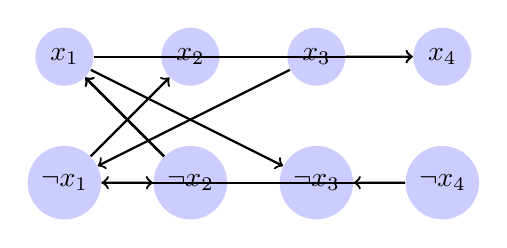
\begin{tikzpicture}
[scale=.8,auto=left,every node/.style={circle,fill=blue!20}]
\node (x1) at (1,3) {$x_1$};
\node (x2) at (3,3)  {$x_2$};
\node (x3) at (5,3)  {$x_3$};
\node (x4) at (7,3) {$x_4$};
\node (nx1) at (1,1)  {$\neg x_1 $};
\node (nx2) at (3,1)  {$\neg x_2 $};
\node (nx3) at (5,1)  {$\neg x_3 $};
\node (nx4) at (7,1)  {$\neg x_4 $};
\tikzset{EdgeStyle/.style={->}}
\Edge(nx1)(nx2)
\Edge(nx2)(x1)
\Edge(x1)(nx3)
\Edge(x3)(nx1)
\Edge(nx1)(x2)
\Edge(nx2)(x1)
\Edge(x3)(x4)
\Edge(nx4)(nx3)
\Edge(x1)(x4)
\Edge(nx4)(nx1)
\end{tikzpicture}\\
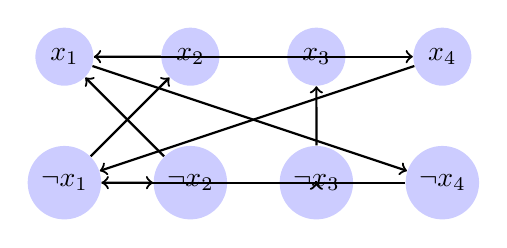
\begin{tikzpicture}
[scale=.8,auto=left,every node/.style={circle,fill=blue!20}]
\node (x1) at (1,3) {$x_1$};
\node (x2) at (3,3)  {$x_2$};
\node (x3) at (5,3)  {$x_3$};
\node (x4) at (7,3) {$x_4$};
\node (nx1) at (1,1)  {$\neg x_1 $};
\node (nx2) at (3,1)  {$\neg x_2 $};
\node (nx3) at (5,1)  {$\neg x_3 $};
\node (nx4) at (7,1)  {$\neg x_4 $};
\tikzset{EdgeStyle/.style={->}}
\Edge(nx1)(x2)
\Edge(nx2)(x1)
\Edge(nx1)(nx2)
\Edge(x2)(x1)
\Edge(x1)(x4)
\Edge(nx4)(nx1)
\Edge(x1)(nx4)
\Edge(x4)(nx1)
\Edge(nx3)(nx3)
\Edge(nx3)(x3)
\end{tikzpicture}
\item Prove: if $G$ has strongly connected component containing $x$ and $\bar{x}$ then $I$ has no satisfying assignment. So, $G$ has a strongly connected component containing $x$ and $\bar{x}$. That means there exists a relation in this strongly connected component $x\to y \to z \to ...  \to p \to \bar{x}$ and $\bar{x}\to a \to b \to ... \to c \to x$. Because this relationship exists both ways, they must have the same value, which cannot be, so the 2SAT problem has no solution. i.e. if $x$ is true, then every term thereafter has to be true. If $x$ is false, every term thereafter must be false. If it did go false$\to$false$\to$true$\to$..., then the converse would have to go true$\to$true$\to$false at some point, but true $\to$ false isn't true. Therefore, $x\iff \bar{x}$ so there would be no solution
\item If none of $G$'s strongly connected components contain both a literal and its negation, then I must be satisfiable. Start with an arbitrary vertex such that $v\to \neg v$ is not an edge (there must be at least one). All nodes reachable by $v$ a value of true. This is valid because if there were paths from $v\to u$ and $v\to \neg u$ then by symmetry there would have to be a path $u\to \neg v$ by how we constructed the graph, which contradicts our initial assumption because $v\to \neg v$ and $\neg v \to v$ in this case. Now that we have assignments for every $u$ reachable by $v$, we can restart this process for a new $v$, which must always exist because of our initial assumption. Continue this process until all literals have an assigned value.
\item There has to be a linear time solution because I just proposed one -- first, construct the directed graph and find its strongly connected components, both of these are linear time (wikipedia suggests Kosaraju's algorithm, Tarjan's algorithm or the path-based strong component algorithm). Next, if any of the components contain a literal and its negation, then conclude no answer (in linear time). Now we keep picking arbitrary nodes and assigning values to each node we visit, visiting each node exactly once -- therefore, we assign the values to the literals and their negations in linear time as well and have come up with a solution to the problem. 
\end{enumerate}
\newpage
\item
\begin{enumerate}
\item In the one dimensional case, we are given $n$ coordinates that fall on a line. If we sort the antennas according to $x$ coordinate, taking $O(n\log(n))$ time, we can then go through each of the dropped calls and do a binary search to find the antenna that dropped that particular call. Binary search takes $O(\log(n))$ and we have to do $n$ of them, so the total running time is $O(n\log(n))$
\item For all of the points (centers of circles and reported locations), find the median $x$ coord ($O(\log(n))$), draw a vertical line $l$ through it, call the subroutine the on the left and right sides -- $T(n)=2T(n/2)+C$. Now we have to determine how long it takes, once we get the results of the subroutine calls to match the unmatched locations on one side with the antennas on the other side. Sort all of the antennas according to $y$ coordinate, taking $O(n\log(n))$, filtering all of them that have a distance to $l$ greater than their radius (can't possible be responsible for a dropped call on the other side of the line). Now that we have it sorted, we can do a binary search through the antennas for each unpaired lost call. We have do to $O(n)$ of these, each taking $O(\log(n))$ time, so the total time to pair them is $O(n\log(n))$. This leads to a total time $T(n)=2T(n/2)+O(n\log(n))=O(n\log^2(n))$ as shown in homework 3.
\item We have to keep the list sorted by $y$ coordinate at all times. That will get rid of one of our $O(n\log(n))$ during our recursion. This shouldn't be that hard. Now that we have a sorted list, we have to pair missed calls with antennas in $O(n)$ time. We can do this by noticing something about the nature of the problem. Only one antenna can cover the area across $l$ at any given $y$ coordinate. Therefore, if we start at the highest (or lowest) value of $y$ and work our way down, as long as we keep a reference for the current antenna on both sides of the line that covers the area on the opposite side of the line (if any), then we can pair up each missed call in order, without searching for each one. I.e. this antenna, whose center is on the left of $l$ is currently covering the area to the right of the line, so if we get a missed call to the right of the line, check if it belongs to that antenna, if it doesn't then keep track of the missed call and when you get the next antenna that crosses the line, if it doesn't cover that missed call then you can declare it unpaired -- this works because an antenna that is further away can't possibly cover it (it would have to overlap with one of the two that were closer). Note, only one antenna can cross the line at once because they don't overlap (can't have a left antenna cover right side and right antenna cover the left side simultaneously), but this doesn't complicate the algorithm. This requires only one traversal of the entire list, $O(n)$, and so the time complexity at each step of the recursion is $O(n)$ and the total recurrence $T(n)=2T(n/2)+O(n)=O(n\log(n))$
\end{enumerate}
\end{enumerate}
\end{document}
